\section{\texorpdfstring{Konečné projektivní prostory}{Konečné projektivní prostory}}
% 9 predn

\subsection{KPP zaklady}

\begin{definition}[Konečný projektivní prostor, kolinearita]\label{kpp:kpp}
    $(P,\LP)$ takový, že $P$ je konečná množina bodů a $\LP$ je množinový systém (přímek) na $P$, je konečný projektivní prostor, splňuje-li axiomy A1, A2, A3.

    Dále body $x\neq y\neq z\neq x$ takové, že $x,y,z\in l\in\LP$, nazveme kolineární.

    \begin{itemize}
        \item[(A1)] $\forall x\neq y\in P\exists! l\in \LP: x,y\in l$
		Takové přímce říkáme $xy$.
        \item[(A2)] netrivialita: $\forall l \in \LP: |l| \geq 3$
	\item[(A3)]  $\forall a,b,c: a\neq b\neq c\neq a, \& a,b,c$ nekolineární: $\forall x\in ac, y\in bc\exists z\in ab$ takový, že $x,y,z$ jsou kolineární.

	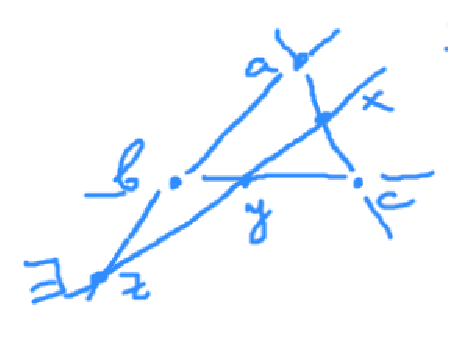
\includegraphics[scale=0.5]{g_0.eps}
    \end{itemize}
\end{definition}

\begin{observation}
	\[ \forall l_1 \ne l_2 \in \LP : |l_1 \cap l_2| \leq 1\]
	Protože jinak pro 2 body ležící v průniku je porušen A1.
\end{observation}

\begin{definition}[Podprostor]\label{kpp:subspace}
    Je-li $(P, \LP)$ konečná geometrie, pak $U \subseteq P$ je podprostor, jestliže
    \[ \forall x\neq y\in U: xy\subseteq U \]
    Zachovává přímky pro všechny body v podprostoru.
\end{definition}

\begin{note}[Podprostor a KPP]
    Je-li $U\subseteq P$ podprostor, pak $(U,\LP|_U)$ je konečný projektivní prostor.
\end{note}

\begin{lemma}[Průnik podprostorů je podprostor]
    Pro $U,V\subseteq \LP$ je podprostor, pak $U\cap V$ je podprostor.
\end{lemma}
\begin{proof}
	Pro libovolné 2 různé body v průniku, dle definice podprostoru
	\[ x \ne y \in U \cap V \Rightarrow xy \subseteq U, xy \subseteq V \Rightarrow xy \subseteq U \cap V \]
\end{proof}

\begin{observation}[Triviální podprostory]
	$(\{ x \}, \emptyset)$ je KPP protože splňuje všechna tvrzení o přímkách, jelikož žádné nemá.

	Podobně $( \emptyset, \emptyset)$ je KPP, z toho lze udělat disjunktní podprostory.
\end{observation}

\begin{definition}[Obal]
    Buď $A \subseteq P, (P, \LP)$: pak $\langle A \rangle$ je nejmenší podprostor, který obsahuje $A$.

    \[ \langle A \rangle = \bigcap_{\substack{U \text{podpr.}\ P \\ A \subseteq U }} U \]
    Protože platí:
    \[ \forall U \text{podpr.}\ P, A \subseteq U: \langle A \rangle \subseteq U \]
\end{definition}

\begin{lemma}[O přidání prvku do podprostoru]\label{kpp:point_add_sub}
    Buď $S \subseteq P$ podprostor $(P, \LP), a \not\in S$.
    Potom $\langle S \cup \{a\} \rangle = \bigcup_{x\in S}ax$.
\end{lemma}
\begin{proof}
	"$\langle S \cup \{a\} \rangle \supseteq \bigcup_{x\in S}ax$".
	Jelikož obal je podprostor, všechny přímky $ax$ v něm musí být.

	Opačnou inkluzi ukážeme tak, že $AX = \bigcup_{x\in S} ax$ je podprostor.
	Obal je průnikem všech podprostoru, takže pokud průnik obsahuje $AX$ tak nemůže mít nic navíc.
	Neboli $\langle S \cup \{a\} \rangle \subseteq \bigcup_{x\in S}ax$.

	Dle \cref{kpp:subspace} musíme ukázat:
	\[ \forall u \ne v: uv \subseteq AX \]
	Rozbor případů:
	\begin{enumerate}
		\item $u = a \lor v = a$, tak druhý bod leží na nějaké přímce $ax$.
			Triviálně cela přímka $ax \subseteq AX$.
		\item $u \in S \land v \in S$ je splněno dle \cref{kpp:subspace}.
		\item BUNO $(u \in S \iff u = x) \land v \not\in S$.
			Pokud $u \in ax$ triviálně.
			Jinak $u \in ay, y \in S$.
			// TODO finish
		\item $u, v \notin S; u, v \ne a; uv \nsupseteq a$
			Chceme $w \in uv \Rightarrow w \in AX$.

		% predn 9 32:17
		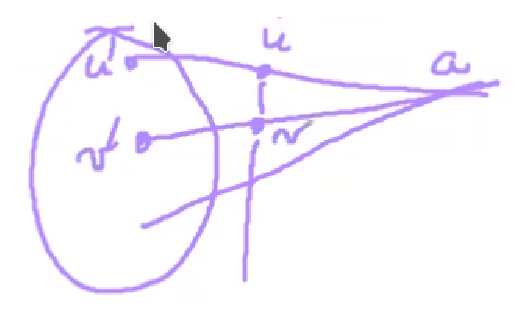
\includegraphics[scale=0.5]{g_1.eps}

		Nechť $u^{\prime} \in au \land u^{\prime} \in S$ analogicky $v^{\prime}$.
		Dle A3:
		\[ \exists y: uv \cap u^{\prime}v^{\prime} \in S \]
		Další 3ce nekolineárních bodů je $u, u^{\prime}, y$.
		Proto $\exists w^{\prime} \in u^{\prime}y \subseteq S$.
		Pak i $w \in w^{\prime}a \Rightarrow w \in AX$.

		% predn 9 37:00
		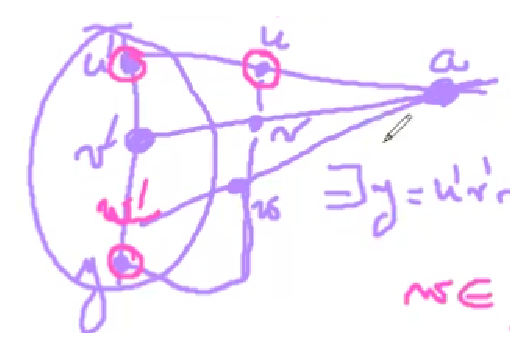
\includegraphics[scale=0.5]{g_25.eps}
	\end{enumerate}
\end{proof}

\begin{lemma}[Sjednocení podprostorů]
    Buďte $S,T \subseteq P$ podprostory $(P, \LP)$.
    Potom
    \[ \langle S \cup T \rangle = \bigcup_{\substack{ s\in S \\ t\in T \\ s\neq t}} st \]
\end{lemma}
\begin{proof}
	Označme $\bigcup_{\substack{ s\in S \\ t\in T \\ s\neq t}} st = SUT$.
	Triviálně platí: $SUT \subseteq \langle S \cup T \rangle$.

	Pro rovnost stačí ukázat že SUT je podprostor.
	Triviální případy:
	\begin{enumerate}
		\item $a \in S \land b \in S$ je splněno dle \cref{kpp:subspace}.
			Analogicky pro $T$.
		\item $a \in S \land b \in T$ dle konstrukce SUT.
		\item $a \in S \land b \in rp, r \in S, p \in T$ jako v \cref{kpp:point_add_sub}.
	\end{enumerate}

	Netriviální případ:
	\[ u \in s_1t_1: s_1 \in S, t_1 \in T \land v \in s_2t_2: s_2 \in S, t_2 \in T \]
	Pokud by $s_1 = s_2 \lor t_1 = t_2$ tvrzení platí z \cref{kpp:point_add_sub}.

	Chceme
	\[ \forall x \in uv \exists a, b: a \in S, b \in T: x \in ab \]
	Kroky:
	\begin{enumerate}
		\item podíváme se na body $s_1, u, v$:
			\[ t_1x \cap s_1u = t_1 \land t_1x \cap uv = x \stackrel{A3}{\Rightarrow} \exists y: t_1x \cap s_1v = y \]
		% predn 9 46:53
		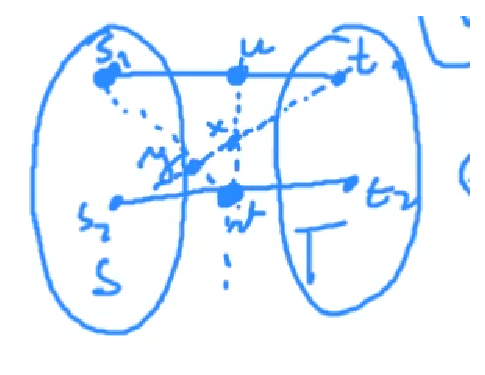
\includegraphics[scale=0.4]{g_2.eps}
	\item podíváme se na body $s_1, s_2, v$:
		\[ t_2y \cap s_2v = t_2 \land t_2y \cap s_1v = y \stackrel{A3}{\Rightarrow} \exists z \in S: t_2y \cap s_1s_2 = z \]
		% predn 9 48:26
		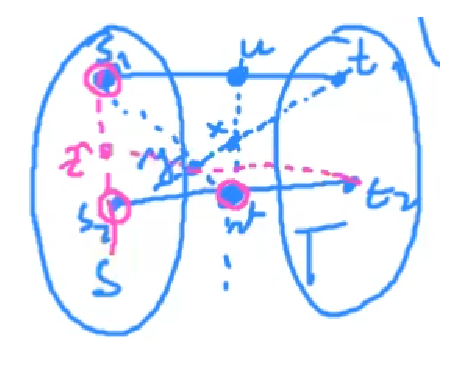
\includegraphics[scale=0.4]{g_3.eps}

	\item podíváme se na body $t_1, t_2, y$:
		\[ zx \cap yt_1 = x \land zx \cap t_2y = z \stackrel{A3}{\Rightarrow} \exists q \in T: t_1t_2 \cap zx = q \]
		% predn 9 50:19
		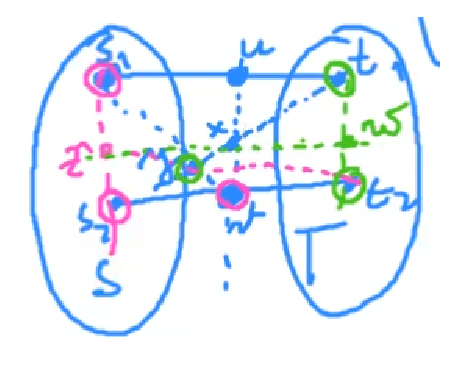
\includegraphics[scale=0.4]{g_4.eps}
	\end{enumerate}
	Dohromady $x \in zq$.
\end{proof}

\begin{definition}[Projektivně nezávislá množina]
    Množina $A\subseteq P$ v $(P,\LP)$ je projektivně nezávislá, jestliže
    \[ \forall a\in A: \langle A\setminus \{a\}\rangle\neq\langle A \rangle \]
\end{definition}

\begin{lemma}[Přidání prvku do projektivně nezávislé množiny]\label{kpp:point_add_ind}
	Je-li $A$ projektivně nezávislá \& $b\not\in\langle A\rangle$, pak $A\cup\{b\}$ je projektivně nezávislá.

	Analogie z vektorových prostoru: pokud máme lineárně nezávislé vektory a přidáme vektor který nelze vyjádřit jako lineární kombinaci, tak dostaneme množinu lineárně nezávislých vektorů.
\end{lemma}
\begin{proof}
	Nechť sporem $A\cup\{b\}$ není projektivně nezávislá $\Rightarrow$
	\[ \exists a \in A\cup\{b\}: \langle A\cup\{b\} \setminus \{ a \} \rangle = \langle A\cup\{b\} \rangle \]
	Rozebereme 2 případy:
	\begin{enumerate}
		\item $a = b \Rightarrow \langle A \rangle = \langle A \cup \{ b\} \rangle \Rightarrow b \in \langle A \rangle$ spor s předpokladem.
		\item $a \in A$.
			Nechť $A^{\prime} = A \setminus \{ a \}$.
			Pak
			\[ \langle A^{\prime} \cup \{ b \} \rangle = \langle A \cup \{ b \} \rangle = \langle A^{\prime} \cup \{ b \} \cup \{ a \} \rangle \Rightarrow a \in \langle A^{\prime} \cup \{ b \} \rangle \]
			Pak ale $a$ leží na nějaké přímce mezi $A^{\prime}$ i $\{ b \}$.
			Neboli nastane situace na obrázku
			% predn 9 59:48
			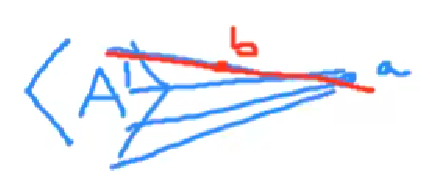
\includegraphics[scale=0.4]{g_5.eps}
			\[ b \in \langle\langle A^{\prime} \rangle \cup \{ a \} \rangle = \langle A \rangle \]
			spor s předpokladem.
	\end{enumerate}
\end{proof}

\begin{observation}[Projektivní nezávislost a generované podprostory]\label{kpp:pr_ind_equiv}
    $A_1,A_2\subseteq P: \langle A_1\rangle=\langle A_2\rangle\Rightarrow \forall x: A_1\cup\{x\}$ je projektivně nezávislá, právě když $A_2\cup\{x\}$ je projektivně nezávislá.
\end{observation}
\begin{proof}
	Tvrzení je symetrické, stačí ukázat:
	\[ A_1\cup\{x\} \text{je pr n }\ \Rightarrow A_2\cup\{x\} \text{je pr n } \]
	$A_1\cup\{x\}$ je pr n $\Rightarrow \langle A_1\cup\{x\} \rangle \ne \langle A_1 \rangle \Rightarrow x \notin \langle A_1 \rangle \Rightarrow x \notin \langle A_2 \rangle \Rightarrow A_2\cup\{x\}$ je pr n.
\end{proof}

\begin{theorem}[O výměně]\label{kpp:exchange}
    Buďte $A,B$ projektivně nezávislé množiny v $(P,\LP)$, $|A| < |B|$.
    Pak existuje $b\in B$ taková, že $A\cup\{b\}$ je projektivně nezávislá.
\end{theorem}
\begin{proof}
	Indukci podle $|A|$ a zpětnou indukci (sestupně) dle $|A \cap B|$.\\
	1) $A = \emptyset \Rightarrow B \ne \emptyset \Rightarrow \exists b \in B \Rightarrow A \cup \{ b \} = \{ b \}$ je triviální případ KPP.

	$A \subseteq B \Rightarrow \exists b \in B \setminus A \Rightarrow A \cup \{ b \}$ je pr nezávislá protože je podmnožinou pr nezávislé.

	2) indukční krok $\exists a \in A \setminus B$.
	Uvažme $A^{\prime} = A \setminus \{ a \}$.
	Jelikož $|A^{\prime}| < |A| < |B|$.
	Dle i.p $\exists b \in B: A^{\prime} \cup \{ b \}$ je pr nezávislá.
	Rozebereme případy:
	\begin{enumerate}
		\item $b \notin \langle A \rangle \stackrel{\cref{kpp:point_add_ind}}{\Rightarrow} A \cup \{ b \}$ je pr nezávislá.
		\item $b \in \langle A \rangle$.
			Označme $A^{\prime\prime} = A^{\prime} \cup \{ b \}$
			$|A^{\prime\prime}| = |A| < |B|$.
			Taky $|A^{\prime\prime} \cap B| > |A \cap B|$.

			Dle i.p (velikost průniku) $\exists c \in B: A^{\prime} \cup \{ c \}$ je pr nezávislá.
			Dal $b \in \langle A \rangle \Rightarrow \langle A^{\prime\prime} \rangle$.
			Dle \cref{kpp:pr_ind_equiv} $A^{\prime} \cup \{ c \}$ je pr nezávislá.

		% predn 9 01:13:00
		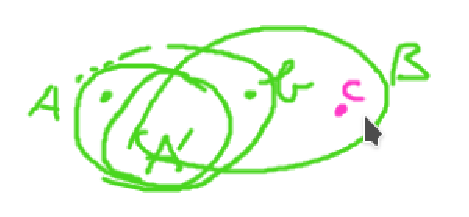
\includegraphics[scale=0.4]{g_6.eps}
	\end{enumerate}
\end{proof}

\begin{definition}[Projektivní báze]
    Projektivní báze je do inkluze maximální projektivně nezávislá množina.
\end{definition}

\begin{consequence}[Projektivně nezávislá množina a báze]\label{kpp:basis}
    Každou projektivně nezávislou množinu lze doplnit na bázi a všechny projektivní báze mají stejnou mohutnost.
\end{consequence}
\begin{proof}
	Nechť máme pr nezávislou $A$.
	KPP je konečný, takže i \# pr nezávislých je konečný.
	Vezmeme největší $B$ pr nezávislou.
	Pak buď $|A| = |B| \Rightarrow A$ je maximální je pr báze.

	Nebo $|A| < |B| \stackrel{\cref{kpp:exchange}}{\Rightarrow} \exists b \in B: A \cup \{ b \}$ je pr nezávislá.
	Můžeme postupovat dokud $|A| < |B|$.
\end{proof}

\begin{definition}[Dimenze]
    $\dim_P S=|B|-1$, kde $B$ je projektivní báze $S$.
\end{definition}

\begin{note}[O dimenzi]
    \begin{itemize}
        \item $\dim_P(\{a\},\emptyset)=0$
        \item $\dim_P(\emptyset, \emptyset)=-1$
        \item $\dim_P(\text{přímka})=2-1=1$.
		2 body tvoří pr nezávislou množinu, 3 již určuji stejnou přímku.
        \item Vezmeme 3 pr nezávislé body jejich obal je KPR. Pak $\dim_P(\text{KPR})=2$
		Taky ale libovolný podprostor s $\dim_P = 2$ je KPR.
    \end{itemize}

    Důsledkem je, že všechny přímky v KPP mají stejnou mohutnost.

    % predn 9 01:28:09
    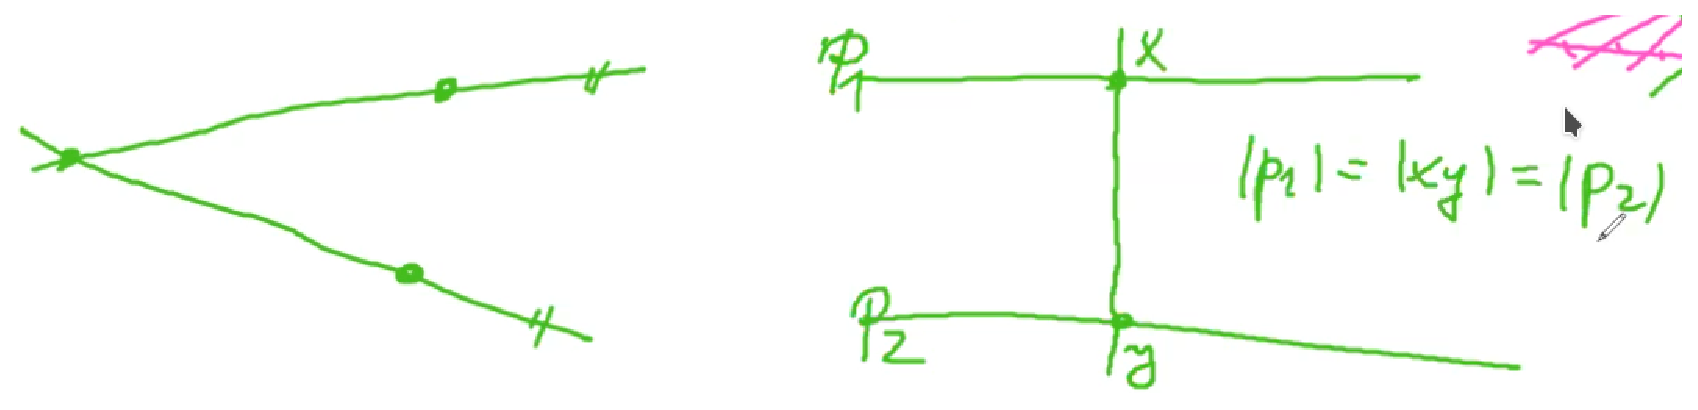
\includegraphics[scale=0.4]{g_7.eps}
\end{note}

% 10 predn
\begin{theorem}[O dimenzi průniku a spojení]\label{kpp:dim_join_inter}
    Buďte $U,V$ podprostory $(P,\LP)$.
    Pak
    \[ \dim_P(U \cap V) + \dim_P(\langle U \cup V \rangle) = \dim_P(U)+\dim_P(V) \]
\end{theorem}
\begin{proof}
	Z uzavřenosti na podprostory, $U \cap V$ je podprostor.
	Z \cref{kpp:basis} má bázi $A$.

	Analogicky má bázi $\langle U \cup V \rangle$.

	Doplníme dle \cref{kpp:exchange} $A$ na bázi $B: \langle B \rangle = U$ a taky na $C: \langle C \rangle = V$.
	$ A \subseteq B, A \subseteq C$.

	Označme:
	\[ \dim_P (U) = u, \dim_P (V) = v, \dim_P (U \cap V) = w \]
	Taky víme
	\[ |B| = u + 1, |C| = v + 1, |A| = w + 1 \]
	\paragraph{Pozorování 1} $B \cup C$ je pr nezávislá množina a generuje $\langle U \cup V \rangle$.
	Vezmeme libovolný $x \in \langle U \cup V \rangle$ tak leží na přímce $ab: a \in U, b \in V$.
	Taky $a, b$ leží na přímkách spojujících 2 body z bázi.
	Najdeme přímku spojující bod z bázi $U$ a bázi $V$ takovou že obsahuje $x$.

    	% predn 10 35:00
    	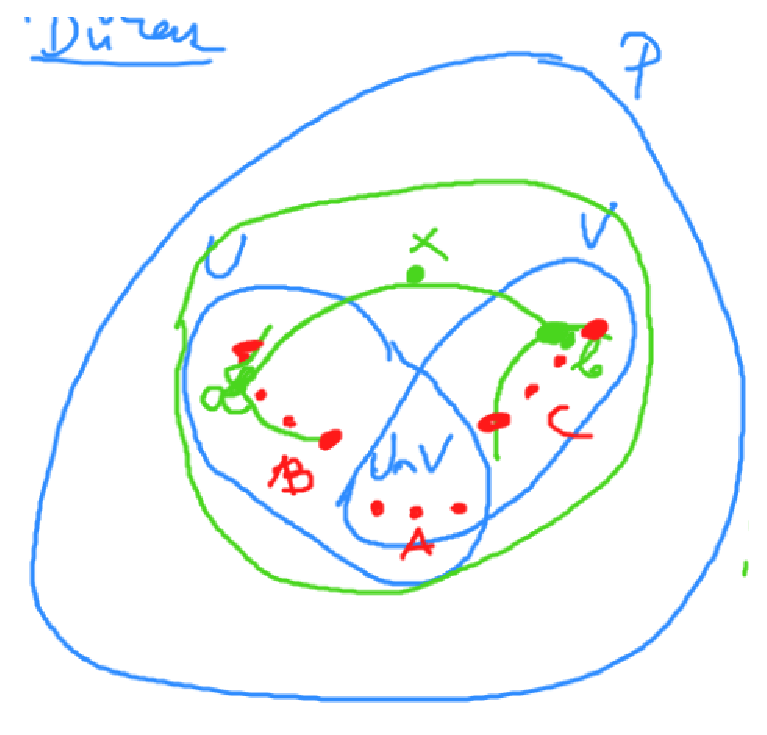
\includegraphics[scale=0.3]{g_9.eps}

	Nechť sporem $B \cup C$ není pr nezávislá množina, pak jeden bod můžeme zahodit.
	\[ \exists a \in C: \langle B \cup C \rangle = \langle (B \cup C) \setminus \{ a \} \rangle \]
	Nutně $a \in C \setminus B$, označme $C_1 = C \setminus \{ a \}$.
	Pak
	\[ \langle B \cup C \rangle = \langle (B \cup C) \setminus \{ a \} \rangle = \langle B \cup C_1 \rangle \]

	Najdeme 2 body $x, y: a \in xy$.
	Může nastat pouze případ $x \in U, y \in V$.
	Protože jinak z vlastnosti podprostoru by $a$ leželo na přímce spojující 2 body báze.
	Takže
	\[ a \in xy: x \in U \setminus V, y \in V \setminus U \Rightarrow x \in ya \subseteq V \]
	spor.

    	% predn 10 39:40
    	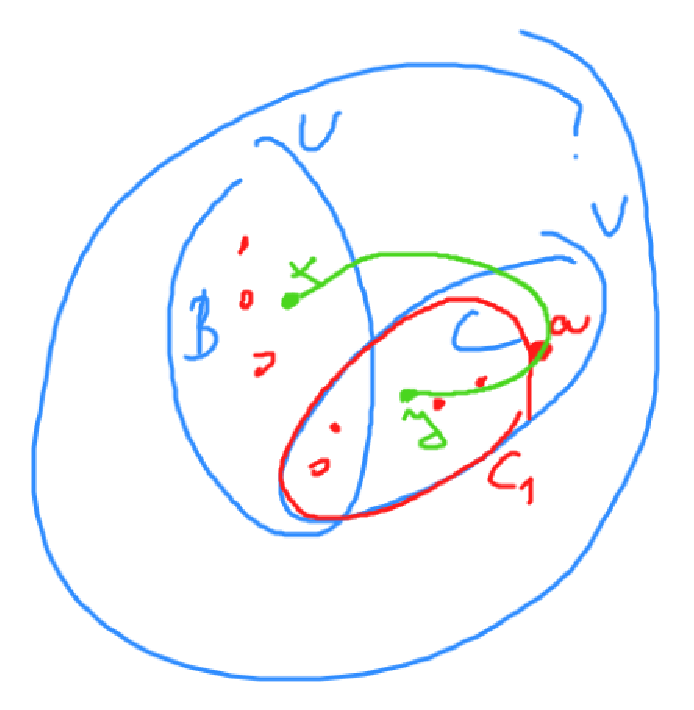
\includegraphics[scale=0.3]{g_10.eps}

	Znovu napíšeme rovnici dimenzi:
	\[ w + \dim_P(\langle U \cup V \rangle) = u + v \]
	Navíc $|B \cup C| - u + 1 + v + 1 - (w + 1) = u + v - w $.
	Pak $\dim_P (B \cup C) = u + v - w$ a dostáváme rovnost.
\end{proof}

\begin{observation}\label{kpp:subspace_dim}
	$U$ je podprostor KPP $P$ a $\dim_P(U) = \dim_P(P) \Rightarrow U = P$.
\end{observation}
\begin{proof}
	Sporem nechť $U \ne V \Rightarrow \exists x \in P \setminus U \Rightarrow x$ je pr nezávislý na bázi $U$.
	Pak
	\[ \dim_P(\langle U \cup \{ x \} \rangle) = \dim_P U + 1 \leq \dim_P P = \dim_P U \]
	spor jak vyšitý.
\end{proof}

\begin{theorem}[Modularita]
    Nechť $A,B,C$ jsou podprostory v $(P, \LP)$ taková, že $B \subseteq A$.
    Pak
    \[ A \cap (\langle B \cup C \rangle) = \langle B \cup (A \cap C) \rangle \]
\end{theorem}
\begin{proof}
	\[ B \subseteq A \& B \subseteq \langle B \cup C \rangle \Rightarrow B \subseteq A \cap (\langle B \cup C \rangle) \]
	Podobně
	\[A \cap C \subseteq A \& A \cap C \subseteq C \subseteq \langle B \cup C \rangle \Rightarrow \langle A \cup C \rangle \subseteq A \cap (\langle B \cup C \rangle) \]
	Dohromady
    \[ A \cap (\langle B \cup C \rangle) \supseteq \langle B \cup (A \cap C) \rangle \]

    	% predn 10 47:00
    	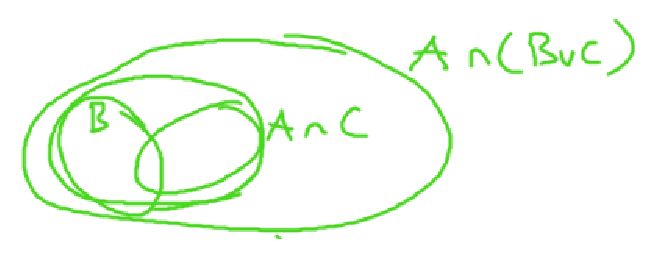
\includegraphics[scale=0.4]{g_11.eps}

	Druhou inkluzi ukážeme pomoci dimenzi a \cref{kpp:subspace_dim}:
	\[ D_1 = \dim_P(A \cap (\langle B \cup C \rangle)) = \dim_P A = \dim_P(\langle B \cup C \rangle) - \dim_P(\langle A \cup B \cup C \rangle) \]
	\[ D_2 = \dim_P(\langle B \cup (A \cap C) \rangle) = \dim_P B + \dim_P(A \cap C) - \dim_P(A \cap B \cap C) \]
	Jelikož $B \subseteq A$:
	\[ D_1 = \dim_P A = \dim_P(\langle B \cup C \rangle) - \dim_P(\langle A \cup C \rangle) \]
	\[ D_2 = \dim_P(\langle B \cup (A \cap C) \rangle) = \dim_P B + \dim_P(A \cap C) - \dim_P(B \cap C) \]
	Taky
	\begin{gather*}
	\dim_P A + \dim_P(B \cap C) + \dim_P(\langle B \cup C \rangle) = \\
	\dim_P A + \dim_P B + \dim_P C = \\
	\dim_P B + \dim_P(A \cap C) + \dim_P(\langle A \cup C \rangle)
	\end{gather*}
	Po úpravách $D_1 = D_2$.
\end{proof}

\begin{consequence}[Průnikem dvou rovin v prostoru je přímka]
    Buď $P,\pi,\sigma: \dim_P P=3, \dim_P\pi = \dim_P\sigma=2, \pi\neq\sigma\Rightarrow \pi\cap\sigma$ je přímka -- $\dim_P(\pi\cap\sigma)=1$.
\end{consequence}
\begin{proof}
	$\langle \pi \cup \sigma \rangle = P$.
	\[ \dim_P(\pi \cap \sigma) = \dim_P \pi + \dim_P \sigma - \dim_P (\langle \pi \cup \sigma \rangle) = 2 + 2 - 3 = 1 \]
\end{proof}

\begin{definition}[Izomorfizmus KPP $\pi \cong \sigma$]
	\[ \exists f: \pi \to \sigma: x, y, z \in l \in \LP_1 \iff f(x), f(y), f(z) \in \LP_2 \]
	kde $f$ je bijekce.
\end{definition}

\begin{theorem}[Roviny si jsou podobné]
    Buď $(P,\LP)$, s $\pi,\sigma$ rovinami v $P$.
    Pak $\pi\cong\sigma$.
\end{theorem}
\begin{proof}
	Víme $\dim_P(\pi \cap \sigma) \leq 2$, pak
    \begin{enumerate}
        \item $\dim_P(\pi \cap \sigma) = 1$ v průniku je přímka.
		Vezmeme $x \in \langle \pi \cup \sigma \rangle \setminus (\pi \cup \sigma)$
		Uvažme
		\[ \forall y \in \pi: xy \cap \sigma = x^{\prime} \]
		Bod existuje protože
		\[ \dim_P xy \cap \sigma = \dim_P xy + \dim_P \sigma - \dim_P(xy \cup \sigma) = 1 + 2 - 3 = 0 \]
		Různým bodům $x$ naleží různé body $x^{\prime}$ protože jinak by byl porušen axiom o 1 přímce.

    	% predn 10 01:11:00
    	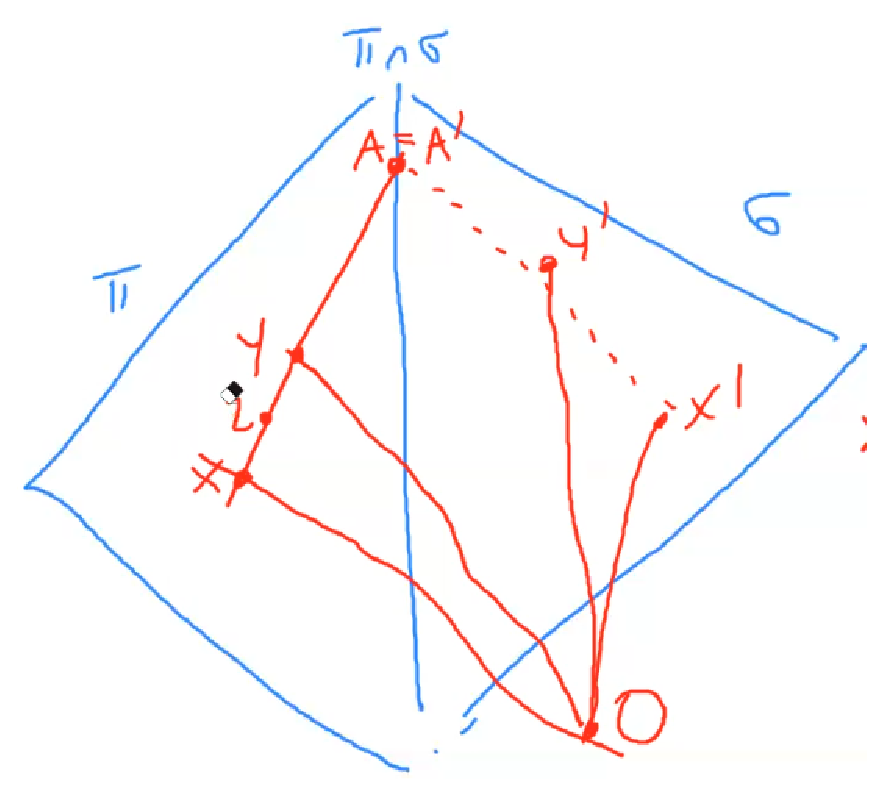
\includegraphics[scale=0.4]{g_12.eps}

	Zbývá ukázat $xy \cap (\pi \cap \sigma = A) \Rightarrow y^{\prime} \in A^{\prime}x^{\prime}$.
	Plyne z A3, dle obrázku:

    	% predn 10 01:14:20
    	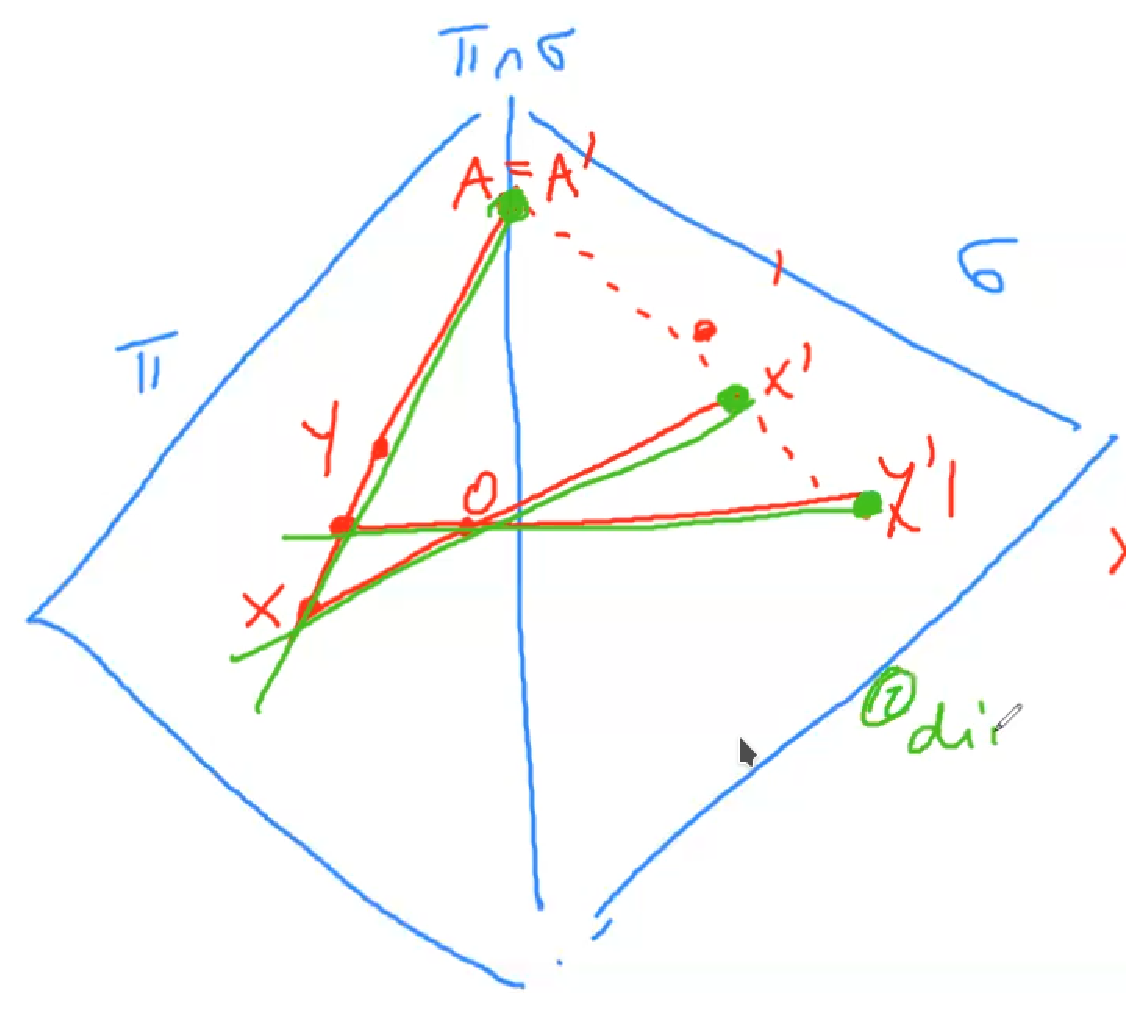
\includegraphics[scale=0.4]{g_13.eps}

        \item $\dim_P(\pi \cap \sigma) = 0$ v průniku je bod $x$.
		Vezmeme bázi $\pi$ a $\sigma$.
		Pak vezmeme $y \in$ bázi $\pi$, $z \in$ bázi $\sigma$ a bod $x$.
		Nechť $\langle \{ x, y, z \} \rangle = \tau$.
		\[ \dim_P \pi \cap \tau = 1 \& \dim_P \sigma \cap \tau = 1 \]
		dle předchozího případu $\pi \cong \tau \cong \sigma$.
	\item $\pi \cap \sigma = \emptyset$.
		Sestavíme $\tau_1$ jako 2 body z bázi $\pi$ a jeden bod z bázi $\sigma$.
		Opačně $\tau_2$ jako 2 body z bázi $\sigma$ a jeden bod z bázi $\pi$.
		Pak
		\[ \dim_P \pi \cap \tau_1 = 1 \& \dim_P \sigma \cap \tau_2 = 1 \& \dim_P \tau_1 \cap \tau_2 = 1 \]
		Takže $\pi \cong \tau_1 \cong \tau_2 \cong \sigma$.
    \end{enumerate}
\end{proof}

\subsection{Singerova konstrukce, Veblen–Young věta}

% 10 predn
\begin{example}
	Nechť $q = p^r$ taky $n \geq 3 \in \N$.
	Uvažme $GF(q)^{n + 1}$, pak body jsou lineární obaly jednotlivých vektorů:
	\[ P = \{ \langle u \rangle |\ u \in GF(q)^{n + 1} \setminus \{ 0 \} \} \]
	Přímky budou všechny podprostory dimenze 2:
	\[ \LP = \{ \langle u, v \rangle |\ u,v LN \in GF(q)^{n + 1} \} \]
	Označme přímky určené vektory $u, v := l_{u, v}$.

	Ověříme axiomy \cref{kpp:kpp}:
	\begin{enumerate}
		\item $|l_{u, v}|$.
			Lineární kombinace dvou vektorů je tvaru $\alpha u + \beta v$.
			Kde $\alpha, \beta \in GF(q)$, neboli $q$ možnosti zvolit každý.
			Musíme ale zahodit kombinaci která dává 0 vektor.
			Vždy ale $q - 1$ násobku stejného vektoru je dle definice stejný bod.
			\[ \# = \frac{q^2 - 1}{q - 1} = q + 1 \]
			Toto $q$ bude řad prostoru.
		\item z konstrukce $\forall u, v LN \exists!$ přímka $l: \langle u \rangle, \langle v \rangle \in l$.
		\item Nechť $u, v, w$ jsou LN vektory.
			Vezmeme $a, b$ ležící na přímce $vu, uw$:
			\[ a = \alpha u + \beta v, b = \gamma u + \delta w \]
			Chceme $xa + yb = rv + sw$.
			\begin{gather*}
				x(\alpha u + \beta v) + y(\gamma u + \delta w) = rv + sw \\
				x \alpha + y \gamma = 0 \\
				x \beta = r \\
				y \delta = s
			\end{gather*}
			Soustava má řešení.
	\end{enumerate}
\end{example}

\begin{theorem}[Singerova konstrukce]
    Existuje-li $(P,\LP)$ KPP řádu $q$ dimenze $n$, pak existuje cyklický $(\frac{q^{n+1}-1}{q-1},\frac{q^n-1}{q-1},\frac{q^{n-1}-1}{q-1})$-SBIBD.
\end{theorem}
\begin{proof}
	$V = P$, $\B = $ nadroviny v $(P, \LP) = $ podprostory $\dim = n - 1$.
	Které vzniknou tak, že ve vektorovém prostoru vezmeme podprostor $\dim = n$.
	\[ |V| = |P| = \frac{q^{n + 1}}{q - 1} = q^n + q^{n - 1} + \ldots + 1 \]
	Velikost nadroviny $H \subseteq P: |H| = \frac{q^n - 1}{q - 1} = q^{n - 1} + q^{n - 2} + \ldots + 1$.

	Nechť $H_1, H_2$ jsou podprostory KPP, které vznikli z podprostoru VP $U_1, U_2$.
	Pak
	\[ \dim(U_1 \cap U_2) = n - 1 \Rightarrow |U_1 \cap U_2| = q^{n - 1} \]
	Jelikož v průniku podprostorů VP je vždy 0 vektor a $q - 1$ jsou násobky stejného vektoru neboli stejného bodu v KPP.
	Takže
	\[ |H_1 \cap H_2| = \frac{q^{n - 1} - 1}{q - 1} \]
	Nadrovin je tolik, kolik je podprostoru v VP.
	Každý podprostor VP je určen lineární rovnici, jejichž počet je roven $\dim$.
	Neboli
	\[ |B| = \frac{q^{n + 1}}{q - 1} = |V| = |P| \]

	V matici incidence $A$ vzniklého množinového systému každé 2 sloupečky mají stejný \# 1.
	% todo tady nechapu argument proc transpozice a radky misto transpozice a sloupce
	Pokud matici transponujeme, tak řádky mají stejný počet 1.
	Neboli $A$ je matice symetrického BIBDu a:
	\[ |H_1 \cap H_2| = \frac{q^{n - 1} - 1}{q - 1} = \lambda \]

    	% predn 10 21:00
    	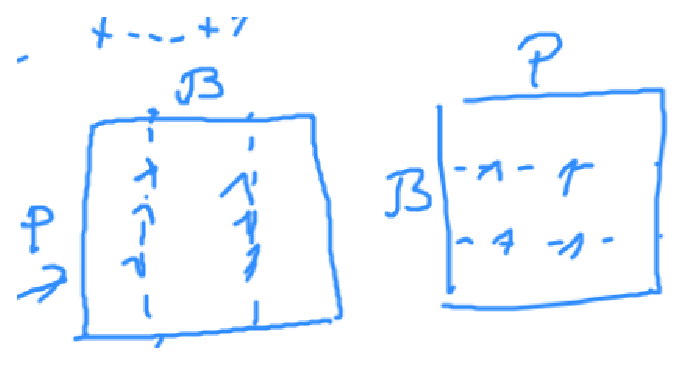
\includegraphics[scale=0.4]{g_8.eps}

	Takže množinový systém je cyklický $(\frac{q^{n+1}-1}{q-1},\frac{q^n-1}{q-1},\frac{q^{n-1}-1}{q-1})$-BIBD.
	Cyklický BIBD znamená, že existuje automorfismus (neboli permutace) který je jediný cyklus.
	Permutace bloků taky bude jediný cyklus.
\end{proof}

\begin{theorem}[KPP $\exists$ BIBD]
    Buď $(P,\LP)$ konečný projektivní prostor řádu $q$ a dimenze $n$.
    Pak jeho nadroviny tvoří symetrický $(\frac{q^{n+1}-1}{q-1},\frac{q^n-1}{q-1},\frac{q^{n-1}-1}{q-1})$-BIBD.
\end{theorem}
\begin{proof}
	Zkontrolujeme vlastnosti BIBDu indukci dle dimenze prostoru, základní případ KPR.
    \begin{enumerate}
	    \item $|P| = q^n + q^{n - 1} + \ldots + 1 = \frac{q^{n+1}-1}{q-1}$.

		    Indukční krok: nechť $H$ podprostor $P$.
		    Dle i.p $|H| = q^{n - 1} + q^{n - 2} + \ldots + 1$.
		    Vezmeme $x \in P \setminus H$, vytvoříme podprostor spojením každého bodu $h \in H$ s $x$ přímkou $xh$, dle \cref{kpp:point_add_sub}.
		    Na každé z těchto přímek je dalších $q$ bodů.
		    Neboli
		    \[ |P| = q \cdot |H| + 1 = q(q^{n - 1} + q^{n - 2} + \ldots + 1) + 1 = q^n + q^{n - 1} + \ldots + 1 \]
	    \item \# nadrovin.
		    Nechť znovu $H, A$ nadroviny: $H \cap A = U$
		    \[ \dim_P H \cup A = n \stackrel{\cref{kpp:dim_join_inter}}{\Rightarrow} \dim_P U = n - 2 \]
		    $U$ je nadrovina v $H$ taky $U$ je průnikem $H$ s $q$ dalšími nadrovinami.
		    $A$ vznikne přidáním přímek mezi 1 bod mimo průnik a $U$.
		    \[ |P \setminus H| = (q^n + q^{n - 1} + \ldots + 1) - (q^{n - 1} + q^{n - 2} + \ldots + 1) = q^n \]
		    Analogicky
		    \[ |H \setminus U| = q^{n - 1} \]
		    Pokud zafixujeme $U$, tak ho lze doplnit na nadrovinu $\frac{q^n}{q^{n - 1}}$ způsoby.
		    Dle i.p $H$ má $(q^{n - 1} + q^{n - 2} + \ldots + 1)$ nadrovin.
		    Z nich vznikne
		    \[ q(q^{n - 1} + q^{n - 2} + \ldots + 1) + \text{sama}\ H = q^n + q^{n - 1} + \ldots + 1 \]
	    \item Vezměme bod $X \in H$.
		    Každá další nadrovina, která bod X obsahuje, protíná $H$ v prostoru projektivní dimenze $(n - 2)$, tento průnik je tedy nadrovina v $H$ obsahující bod $X$.
		    Podle indukčního předpokladu je takovýchto nadrovin $q^{n-2} + q^{n-3} + \ldots + 1$, a podobně jako v předchozím bodě, každá z nich vznikla jako průnik s $q$ možnými nadrovinami v $P$.
    \end{enumerate}
\end{proof}

% 11 predn
\begin{theorem}[KPP dimenze alespoň 3 mají Desargovskou vlastnost]
    Konečné projektivní prostory dimenze alespoň 3 mají Desargovskou vlastnosti.
\end{theorem}
\begin{proof}
	Rozbor případu:
	\begin{enumerate}
		\item $O, A, B, C$ neleží v jedné rovině.
			Taky to znamená, že
			\[ \pi = \langle A, B, C \rangle \ne \langle A^{\prime}, B^{\prime}, C^{\prime} \rangle = \sigma \]
			Všechny body na obrázku leží v 3-dim podprostoru.

    	% predn 11 05:00
    	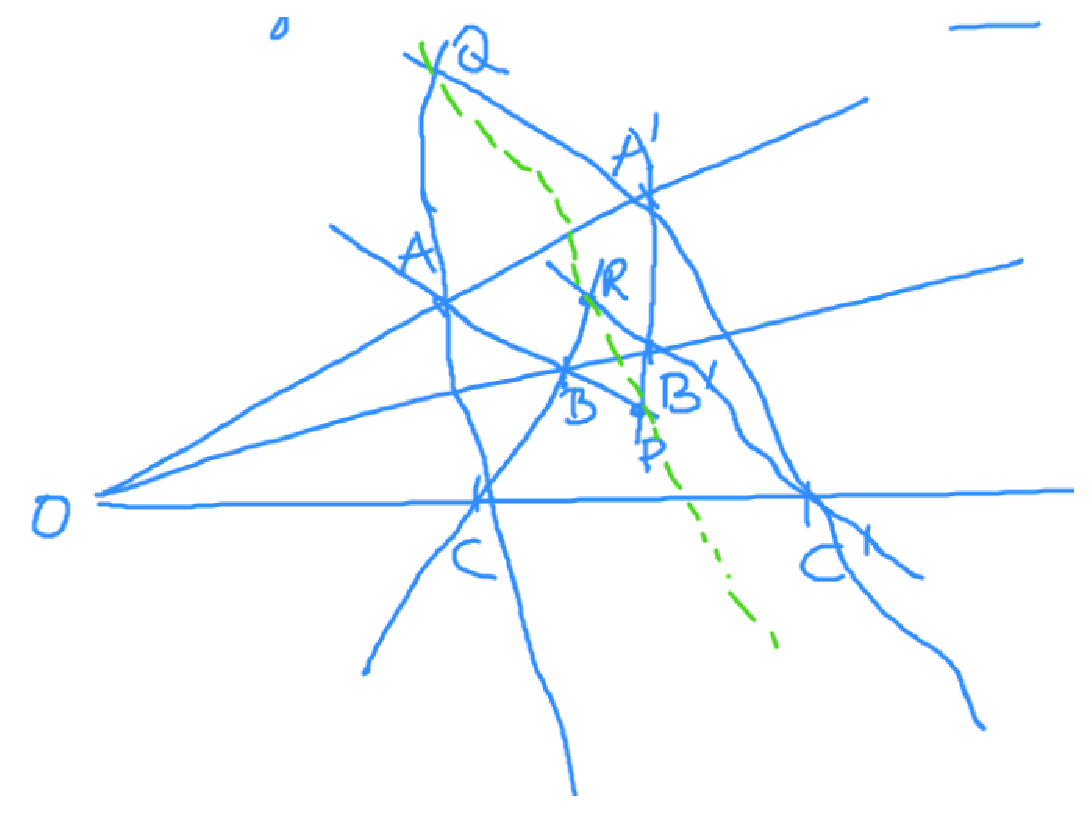
\includegraphics[scale=0.2]{g_14.eps}

	Protože např $OA^{\prime}C^{\prime}$ tvoří rovinu.
	Přidáním bodu $B$ dimenze se zvedne o 1.
	Konečné bod $B^{\prime}$ vytvoří 3d prostor

	Proto
	\[ \dim_P(\pi \cap \sigma) = \dim_P \pi + \dim_P \sigma - \dim_P(\langle \pi \cup \sigma \rangle) = 2 + 2 - 3 = 1 \]
	Bod $P \in AB \& P \in A^{\prime}B^{\prime} \Rightarrow \in \pi \cap \sigma$
	Podobně $Q, R$.
	Tyto 3 body jsou na hledané přímce.
		\item $O, A, B, C$ leží v jedné rovině $\pi$.
			\begin{enumerate}
				\item Vezmeme 2 body mimo rovinu
			\[ \exists S \notin \pi, B_0 \in SB, B_0 \ne S, B_0 \notin \pi \]
			Pak přímky $SP \cap AB_0 = P_0$.
			Taky $SB^{\prime} \cap OB_0 = B_0^{\prime}$.

			Tvrdíme $P_0, A^{\prime}, B_0^{\prime}$ jsou kolineární.
			Za prvé leží v $SPB^{\prime} \cap OAB_0$.
			\begin{gather*}
			P_0 \in PS \& A^{\prime} \in PB^{\prime} \& B_0^{\prime} \in SB^{\prime} \Rightarrow P_0, A^{\prime}, B_0^{\prime} \in SPB^{\prime} \\
			P_0 \in AB_0 \& A^{\prime} \in OA \& B_0^{\prime} \in OB_0^{\prime} \Rightarrow P_0, A^{\prime}, B_0^{\prime} \in OAB_0
			\end{gather*}

    	% predn 11 05:00
    	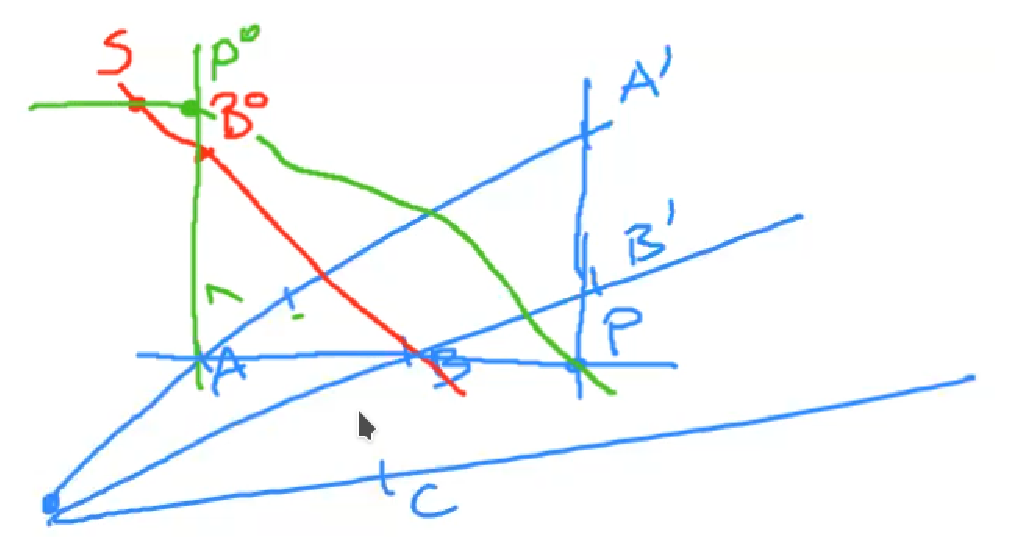
\includegraphics[scale=0.4]{g_26.eps}

				\item Podobně $R_0 = CB_0 \cap RS$.
			Tvrdíme jako výš $R_0, C^{\prime}, B_0^{\prime}$ jsou kolineární.

			\item Tvrdíme jako výš $P_0, R_0, Q$ jsou kolineární.
			Protože
			\begin{gather*}
			P_0, R_0, Q \in AB_0C \cap A^{\prime}B_0^{\prime}C^{\prime} \\
			P_0 \in AB_0 \& R_0 \in CB_0 \& Q = AC \cap A^{\prime}C^{\prime} \Rightarrow Q \in AC \Rightarrow \in AB_0C \\
			P_0 \in A^{\prime}B_0^{\prime} \& R_0 \in C^{\prime}B_0^{\prime} \& Q \in A^{\prime}C^{\prime} \Rightarrow \in A^{\prime}B_0^{\prime}C^{\prime}
			\end{gather*}

			\item Finálně $P, Q, R$ jsou kolineární.
			$P, Q, R \subseteq \pi \cap SP_0R_0$
			\[ P \in SP_0 \& R \in SR_0 \& Q \in P_0R_0 \Rightarrow \in SP_0R_0 \]
			\end{enumerate}
	\end{enumerate}
\end{proof}

\begin{definition}[Automorfismus]
    Bijekce $\alpha: (V,\B)\rightarrow (V,\B)$ taková, že $\forall B\in \B: \alpha[B]\in\B$ je automorfismus.
\end{definition}

\begin{note}[Inverz automorfismu je automorfismus]
    Pro konečné prostory platí, že pro $\alpha$ automorfismus je $\alpha^{-1}$ automorfismus.
\end{note}
\begin{proof}
	$\alpha$ jako permutace prvků je disjunktní sjednocení cyklů.
	Jelikož $\alpha$ je automorfismus, z každého bloku vede právě jedna šipka.
	Nemůže se stát, aby z bloky vedli 2 hrany.
	Taky dokážeme, že do každého bloku vede právě jedna šipka.
	Pro libovolný blok z bijekce platí:
	\[ \exists! A: \alpha(A) = B^{\prime} \]
	V grafu zobrazení $\alpha: \forall u: deg_{out}(u) = 1, deg_{in} \leq 1$.
	Z konečnosti i $deg_{in} = 1$.

    	% predn 11 31:00
    	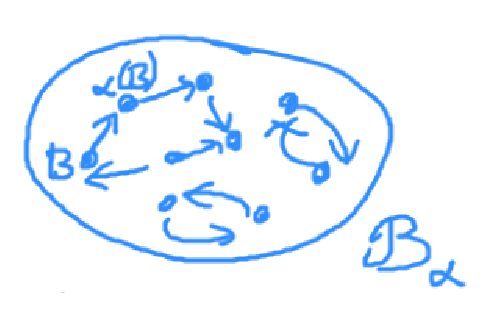
\includegraphics[scale=0.4]{g_15.eps}

	Neboli $\alpha$ na blocích je taky permutace.
	Pokud půjdeme po cyklech zpátky, znovu dostaneme bloky:
	\[ \forall B \in \B: \alpha^{-1}(B) \in \B \]

	Takže automorfismy tvoří grupu.
\end{proof}

\begin{definition}[Kolineace]
    Kolineace je zobrazení $\alpha: V \cup \B \rightarrow V \cup \B$ takové, že $\alpha\upharpoonright V$ je bijekce na $V$, $\alpha\upharpoonright \B$ je bijekce na $\B$ a zachovává incidence
    \[ \forall x \in V, \forall B \in \B: x \in B \Leftrightarrow \alpha(x) \in \alpha(B) \]
\end{definition}

\begin{theorem}[Automorfismy a kolineace]\label{kpp:equiv}
    Nechť pro $(V,\B)$ platí:
    \[ \forall B \in \B: |B| \geq 2 \& \forall x \ne y \in V \exists! B \in \B: x, y \in B \]
    Neboli je to nepravidelný $(|V|, \{ 2, 3, \ldots \}, \lambda = 1)$-BIBD.

    Nechť $\alpha: V\rightarrow V$ je permutace, $\overline{\alpha}: V\cup B\rightarrow V\cup 2^V$ takové, že
    \[ \forall x \in V: \overline{\alpha}(x) = \alpha(x) \]
    a $\overline{\alpha}(B) = \{ \alpha(x): x \in B \}$.
    Pak následující tvrzení jsou ekvivalentní:
    \begin{enumerate}
        \item $\alpha$ je automorfismus
        \item $\overline{\alpha}$ je kolineace
        \item $\alpha$ zachovává kolinearitu:
		\[ \forall x \ne y \ne z \ne x \in V: x, y, z\ \text{kolineární}\ \Rightarrow \alpha(x), \alpha(y), \alpha(z)\ \text{kolineární} \]
    \end{enumerate}
\end{theorem}
\begin{proof}
    \begin{enumerate}
        \item Označme zobrazení na prvcích a blocích jako $\overline{\alpha}$.
		Aby vůbec byla kolineace, musí zachovávat incidence:
		\[ \overline{\alpha}(B) = \{ \alpha(x): x \in B \} \]
		Z vlastnosti automorfismu, zobrazuje blok na blok, neboli je kolineace.
        \item $\overline{\alpha}$ je kolineace což implikuje, že $\overline{\alpha}$ permutace na blocích $\Rightarrow \alpha$ je automorfismus.
        \item z kolinearity
		\[ \forall B \in \B \exists B^{\prime} \in \B: \alpha(B) \subseteq B^{\prime} \]
		Sestrojíme graf, vrcholy jsou bloky, hrany dle předchozího vztahu:
		\[ \B_{\alpha}^C = (\B, \{ BB^{\prime}: \alpha(B) \subseteq B^{\prime}\}) \]
		Z každého vrcholu vychází aspoň 1 hrana.
		Nechť sporem z bloku $B$ máme 2 out hrany.
		Pak $\alpha(B) \subseteq B_1 \cap B_2$, z předpokladu $|B| \geq 2$.
		Takže v průniku jsou 2 body, spor protože každé 2 prvky jednoznačně určuji blok.
		Neboli $\forall u: deg_{out}(u) = 1$.

		Rozdělíme bloky dle velikosti, víme pro hrany z jednoznačnosti $|B| \leq |B^{\prime}|$.
		V rámci skupiny největších bloků $B^{\prime}$ už nemůže být větší, takže $\alpha(B)$ je blok.
		Nechť sporem kdyby ze skupiny menších bloku vedla hrana do větších, tak platí:
		\[ |B_m| < |B| = |B^{\prime}|: \alpha(B) = B^{\prime} \& \alpha(B_m) = B^{\prime} \]
		Z bijekce na prvcích nutně $B_m \subseteq B$, znovu spor s jednoznačnosti bloků určených 2ma prvky.

		Sestupnou indukci dle velikosti bloků dokážeme, že blok se zobrazuje na blok.

    	% predn 11 31:00
    	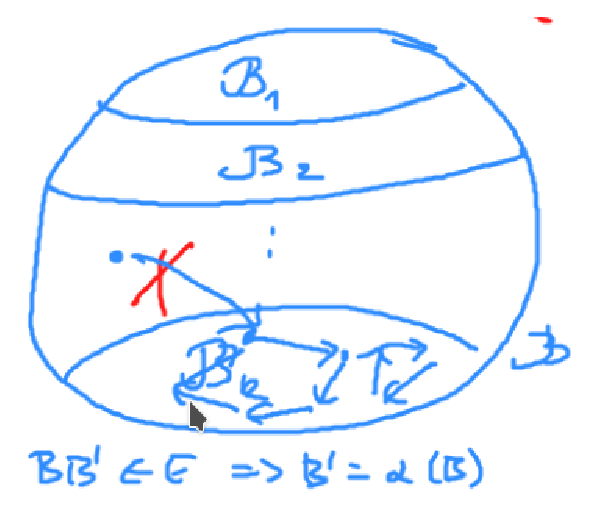
\includegraphics[scale=0.4]{g_16.eps}
    \end{enumerate}
\end{proof}

\begin{agreement}
	Nadále mluvíme o KPP řádu $q \geq 2$ a $\dim_P \geq 2$(většinou $\geq 3$).
\end{agreement}

\begin{note}[Kolineace a obrazy přímek]
    Je-li $\alpha$ kolineace prostoru, pak
    \[ \forall x\neq y\in P: \alpha(xy)=\alpha(x)\alpha(y) \]
\end{note}
%\begin{proof}
%    TODO
%\end{proof}

\begin{definition}[Fixace]
    $A\subseteq P$: $\alpha$ fixuje všechny body $A$, jestliže $\forall x\in A: \alpha(x)=x$

    $l\in\LP: \alpha$ fixuje $l$, jestliže $\alpha[l]=l$.
\end{definition}

\begin{definition}[Centrální kolineace]\label{kpp:centr_kolin}
    Centrální kolineace $(P,\LP)$ je kolineace, pro niž existuje nadrovina $H$ (nazývaná osa kolineace), jejíž všechny body jsou fixované kolineací $\alpha$, a bod $C\in P$ (nazývaný střed kolineace) takový, že všechny přímky jím procházející jsou zobrazením $\alpha$ fixované.

    (Pozor, může nastat $C\in H$ i $C\not\in H$.)
\end{definition}

\begin{lemma}[Kolineace fixující nadrovinu]\label{kpp:kolin_centr_kolin}
    Buď $\alpha$ kolineace fixující všechny body nadroviny $H\subseteq P$.
    Pak existuje $C\in P$ tak, že $\alpha$ fixuje  všechny přímky procházející bodem $C$.

    Ekvivalentně každá kolineace fixující rovinu je nutně Centrální.
\end{lemma}
\begin{proof}~
	%predn 12 05:00
    \begin{enumerate}
	    \item $ \exists C \notin H: \alpha(C) = C$.
		    Každá přímka, která neleží v $H$ ji protíná v 1 bodě.
		    Nechť $P \in H: (CP = g) \cap H = P$.
		    \[ \alpha(g) = \alpha(PC) = \alpha(P)\alpha(C) \stackrel{osa}{=} P\alpha(C) \stackrel{předpoklad}{=} PC \]
		    Neboli každá přímka procházející $C$ je fixovaná.
	    \item $ \forall X \in P \setminus H: \alpha(X) \ne X$.
		    Vezmeme libovolný $Y \notin H$, pak $\alpha(P) \ne P, \alpha(P) \notin H$.
		    Nechť $P\alpha(P) \cap H = C$, dal nějakou přímky která neleží v $H$.
		    Nechť na této přímce je bod $Q \notin H$.

		    \[ PQ \notin H \Rightarrow PQ \cap H = S \]
		    Pak $\alpha: PQS \to \alpha(P) \alpha(Q) \alpha(S) = \alpha(P) \alpha(Q) S$.
		    Takže $\alpha(Q) \in S \alpha(P)$
		    $P, Q$ jsou různé body, proto i přímky $Q\alpha(Q) \ne P\alpha(P)$.
		    Taky leží ve stejné rovině určené přímky $SP, PQ$.
		    Proto $\exists T:= Q\alpha(Q) \cap P\alpha(P)$.
		    Pak
		    \[ \alpha(T) = \alpha(Q\alpha(Q)) \cap \alpha(P\alpha(P)) \]
		    Kvůli tomu, že $H$ osa, $\alpha(PC) = \alpha(P)C = PC \Rightarrow P\alpha(P)$ je fixovaná, analogicky $Q\alpha(Q)$.
		    Neboli
		    \[ \alpha(T) = \alpha(Q\alpha(Q)) \cap \alpha(P\alpha(P)) = Q\alpha(Q) \cap P\alpha(P) = T \]
		    Což implikuje $T = H \cap P\alpha(P)$, protože body mimo $H$ nejsou fixované.
		    Jediný takový bod je ale $C \Rightarrow T = C$.
		    Takže přímka $QC$ je fixovaná $\alpha$.

    	% predn 12 14:40
    	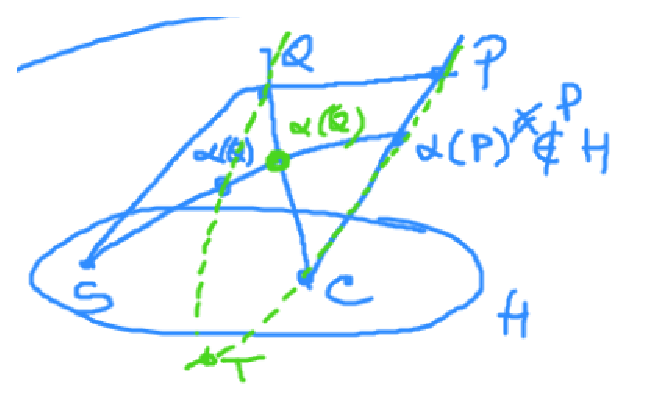
\includegraphics[scale=0.3]{g_18.eps}
    \end{enumerate}
\end{proof}

\begin{lemma}[Rozšíření kolineace]\label{kpp:extension}
    Mějme $q_0\in\LP\rightarrow (P',\LP'), P' = P\setminus g_0$ množinový systém.
    Pak každou kolineaci $\alpha$ množinového systému $(P',\LP')$ je možno rozšířit na kolineaci $\alpha^*$ prostoru $(P, \LP)$ právě jedním způsobem, a tato kolineace fixuje $g_0$.
\end{lemma}
\begin{proof}
	Z původního KPP vznikne množinový systém $(P',\LP')$:
	\[ P' = P\setminus g_0 \& \LP' = \{ l': l' = l \setminus g_0: l \in \LP \} \]
	Potřebujeme dodefinovat $\alpha^*$ pro přímku $g_0$, jinde je shodné s $\alpha$.
	Přímky disjunktní s $g_0$ jsou fixované:
	\[ \forall l \in \LP \cap \LP': l \cap g_0 = \emptyset: \alpha^*(l) = \alpha(l) \]
	Ostatní:
	\[ \forall l \in \LP: l \cap g_0 = x: \alpha^*(l) = \alpha(l') \cup \{ \alpha(x) \} \]
	Problém ale nastane, pokud máme 2 zkrácené, které se protínají s $g_0$ ve stejném bodě.
	Dokážeme že to nejde
	\[ \forall g \ne h \in \LP: g \cap h = p \in g_0 \Rightarrow |\alpha^*(g) \cap \alpha^*(h)| \ne 0 \& \alpha^*(g) \cap \alpha^*(h) \subseteq g_0 \]
    \begin{enumerate}
	\item $q > 2$, takže přímky $g, h$ kromě průniku mají ještě aspoň 3 body.
		    Pak určuji rovinu $H = \langle g \cup h \rangle$.
		    Z velikosti podprostoru, máme ještě nějakou přímku a bod $Q \in H: Q \notin g \cup h$.
		    Vezmeme přímky $Q \in m, n: g,h \cap n,m \ne \emptyset$.
		    Z kolineace kvůli $\alpha(m), \alpha(n)$, $\alpha(g'), \alpha(h')$ jsou ve stejné rovině $\Rightarrow \alpha^*(g) \cap \alpha^*(h)$ taky.
		    Pak $\exists x = \alpha^*(g) \cap \alpha^*(h) \in g_0$.

    	% predn 12 28:30
    	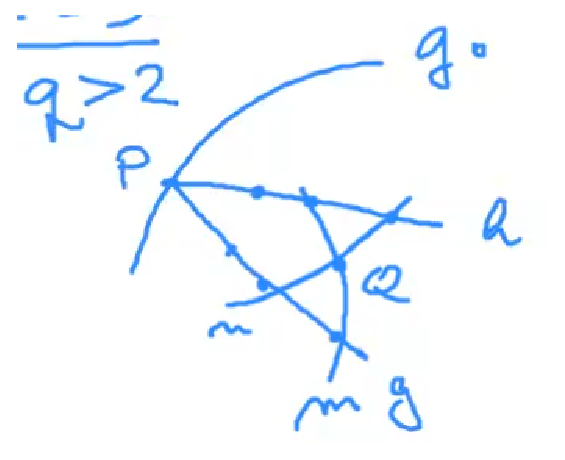
\includegraphics[scale=0.3]{g_19.eps}

	\item $q = 2$, pokud $g_0, g, h$ neleží v jedné rovině.
		Pak stejná úvaha jako v 1).

	\item $q = 2$, pokud $g_0, g, h$ leží v jedné rovině.
		Víme že $\dim_P \geq 3 \Rightarrow \exists m$ která v rovině neleží.
		Použijeme případ 2) pro $m, h, g_0$ a $m, g, g_0$.
	\item $q = 2, \dim_P P = 2 \iff$ Fanova rovina taky platí, důkaz ad hoc.
    \end{enumerate}
\end{proof}

\begin{lemma}[Centrální kolineace tvoří grupu (BD)]
    Centrální kolineace s osou $H$ a středem $C$ tvoří grupu vzhledem ke skládání, jednotkou je identita.
\end{lemma}
\begin{proof}
	Nechť $\Gamma$ je množina centrálních kolineace s osou $H$ a středem $C$.
	Je neprázdná, protože obsahuje identitu.

	$\Gamma$ je uzavřená na kompozice, protože pro libovolné $\alpha, \beta \in \Gamma, \alpha \circ \beta$ fixuje body $H$ a každou přímku procházející bodem $C$.

	Konečné, $\forall \alpha \in \Gamma$ je $\alpha^{-1} \in \Gamma$ protože $\alpha\alpha^{-1} = id$, $\alpha^{-1}$ taky musí fixovat body $H$ a každou přímku procházející bodem $C$.
\end{proof}
% lemma 3.1.2
Source ~\cite[p. 96]{beutelspacher1998projective}.

\begin{lemma}[Vlastnosti centrální kolineace]\label{kpp:centr_kolin_prop}
    Buď $\alpha$ centrální kolineace s osou $H$ a středem $C$. Potom
    \begin{enumerate}
        \item $P\not\in H\cup\{C\}\Rightarrow \forall x: \alpha(x)$ jednoznačně určen bodem $\alpha(P)$ tak, že:
		\[ \alpha(x)=CX\cap F\alpha(P), F=PX\cap H \]
        \item Není-li $\alpha$ identická kolineace, pak každý bod mimo $H\cup \{C\}$ není fixovaný
        \item Centrální kolineace $\alpha$ je jednoznačně určena kteroukoliv dvojicí $P\neq\alpha(P)$.
    \end{enumerate}
\end{lemma}
\begin{proof}
	%\paragraph{
	Pozorování: $P, \alpha(P), C$ jsou kolineární.
	Přímka $\alpha(PC) = PC$ z \cref{kpp:centr_kolin} jako střed.
	Taky ale
	\[ \alpha(PC) = \alpha(P)\alpha(C) \stackrel{střed}{=} \alpha(P) C \Rightarrow \alpha(P) \in PC \]

	Dal $PC \nsubseteq H$, spojení nadroviny a přímky už je nutně celý prostor, proto
	\[ \dim_P H = n - 1 \& \dim_P PC = 1 \Rightarrow \dim_P (H \cap PC) = n - 1 + 1 - n = 0 \]
	V průniku jeden bod.

    \begin{enumerate}
	    \item Vezmeme $X \notin PC$.
		    Přímka $PX \notin H \Rightarrow PX \cap H = F$ bod.
		    \[ X \in FP \Rightarrow \alpha(X) \in \alpha(FP) = \alpha(F)\alpha(P) \stackrel{osa}{=} F\alpha(P) \]
		    Protože $\alpha$ kolineace: $X \in XC \Rightarrow \alpha(X) \in \alpha(XC) \stackrel{střed}{=} XC$.
		    $XC, FP$ jsou různé přímky, proto $\alpha(X) = XC \cap F\alpha(P)$.
		    Taky $X \ne \alpha(X)$ protože přímky $X \in FP, \alpha(X) \in F\alpha(P)$ jsou různé $X \notin F\alpha(P)$.

    	% predn 11 01:24:00
    	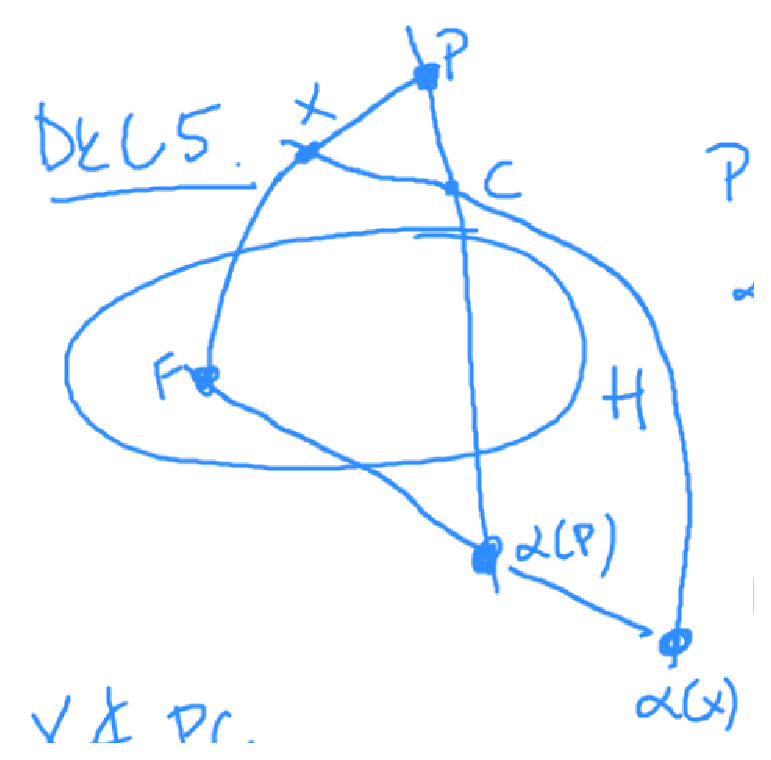
\includegraphics[scale=0.3]{g_17.eps}
\item Vezmeme $X \in PC$, nutně neleží v $H$, protože jinak je fixovaný a je určen jednoznačně.
	Analogicky $X \ne C$.
	Vezmeme libovolný $R \notin PC, H$, přímka $RC$ jednoznačně určuje bod $\alpha(R)$.
	$X \notin RC$, dle 1) $\alpha(X)$ je jednoznačně určen $\alpha(R)$.

	\item Plyne okamžitě z 1).
    \end{enumerate}
\end{proof}

\begin{consequence}[Jednoznanost středu i osy kolineace]
    Je-li $\alpha$ neidentická kolineace, pak její osa i střed jsou jednoznačně určené.
\end{consequence}
\begin{proof}~
	\begin{enumerate}
		\item Osa je jednoznačná.
			Nechť $\alpha$ fixuje 2 nadroviny $H \ne A$.
			Průnik je o 1 dimenze menší, neboli $\exists X, Y \in A \setminus H$ které jsou fixované.
			Spor s \cref{kpp:centr_kolin_prop}.2.
		\item Nechť $H$ je osa.
			Nechť $\alpha$ neidentická kolineace se středy $C_1 \ne C_2 \notin H$.
			Pak spor protože dle \cref{kpp:centr_kolin_prop} žádný další bod kromě $C_1$ není fixovaný.
	\end{enumerate}
    TODO not complete
\end{proof}

%13 predn

\begin{theorem}[Baerova]\label{kpp:baer}
    Buď $H$ nadrovina v Desargovském prostoru $(\mathcal{P},\LP)$ a buďte $P,P', C$ tři různé kolineární body takové, že $P,P\not\in H$.
    Pak existuje právě jedna centrální kolineace $\alpha$ taková, že $H$ je osa, $C$ je střed, $\alpha(P)=P'$.
\end{theorem}
\begin{proof}[Náznak důkazu]
    $\mathcal{P}':=\mathcal{P}\setminus PC$ -- zadefinujeme
    \[ \alpha(x) := \twopartdef{x}{x\in H\cup \{C\}}{FP'\cap CX, F=PX\cap H}{x\not\in H\cup \{C\}} \]
    Toto je jednoznačné, neboť (TODO obrázek).

    % predn 12 40:00
    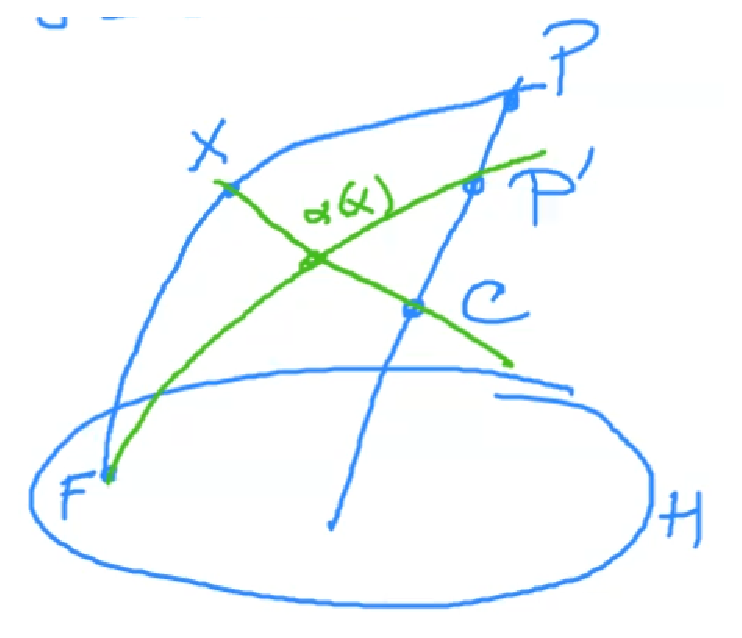
\includegraphics[scale=0.3]{g_20.eps}

    Dokážeme, že $\alpha$ je kolineace v $P'$.
    \begin{enumerate}
	    \item neboť $\alpha$ je bijekce, jelikož máme
		    \[ c \neq x_1 \neq x_2 \neq c\Rightarrow \alpha(x_1)\neq\alpha(x_2) \]
    		\begin{enumerate}
			\item $x_1, x_2, P$ kolineární.

    % predn 12 47:00
    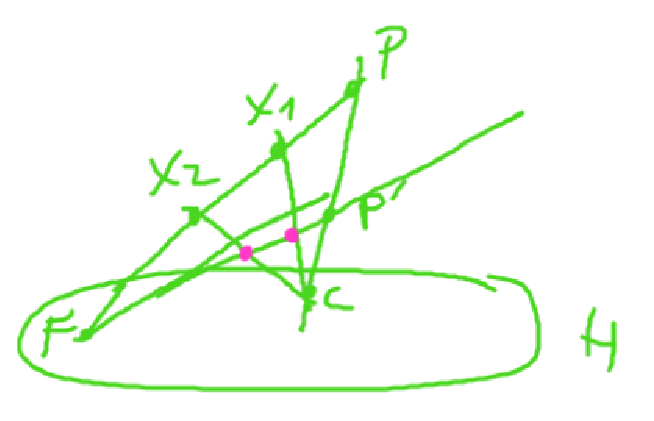
\includegraphics[scale=0.3]{g_21.eps}

    Z obrázku, $\alpha(x_1)\neq\alpha(x_2)$ protože jinak by $Cx_1, Cx_2$ různé přímky by měli 2 společné body.
			\item $x, y, P$ nekolineární.
				\[ Q = xy \cap \alpha(x)\alpha(y) \]
    % predn 12 47:00
    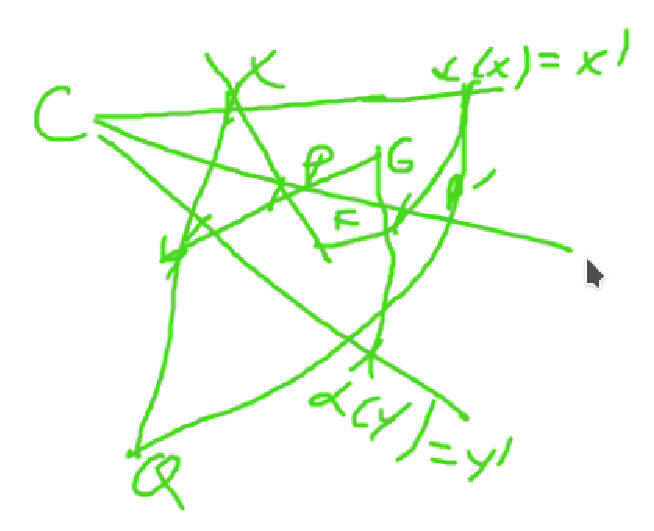
\includegraphics[scale=0.3]{g_22.eps}

    			Na obrázku jsou body jako v definici Desargovské vlastnosti, která platí pro KPP dostatečné velikosti.
			Takže $Q, F, G$ jsou kolineární proto
			\[ \Rightarrow F, G \in H \Rightarrow FG \subseteq H \Rightarrow Q \in H\]

    		\end{enumerate}

		Dohromady odvodíme
		\[ \forall x, y: xy \cap \alpha(x)\alpha(y) \in H \]
		Pokud vezmeme 3 kolineární body, tak z tvrzení výš průnik přímky určené jejích obrazy je stejný bod $F$. Neboli $\alpha$ zachovává kolinearitu.

		Dle \cref{kpp:equiv} $\alpha$ je kolineace.

    % predn 12 57:20
    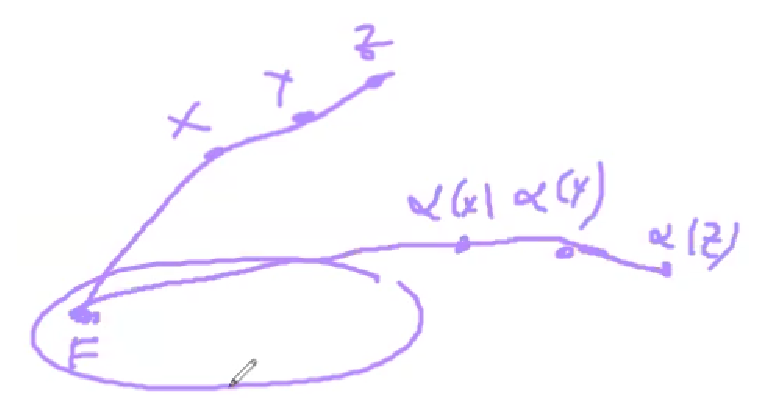
\includegraphics[scale=0.3]{g_23.eps}

	\item použijeme \cref{kpp:extension} pro $\alpha$, čímž dostaneme zobrazení zachovávající kolinearitu pro $P$.
		% todo ref
	\item Z vlastnosti 3 plyne, že všechny další přímky procházející bodem $C$ jsou fixovány.
		Je tedy $C$ střed a $H$ osa kolineace $\alpha^*$.
    \end{enumerate}
\end{proof}

\begin{definition}[Množiny kolineací]
    \begin{itemize}
	\item Množinu kolineací prostoru značíme $\mathrm{Col}(P)$.
        \item Množinu centrálních kolineací označíme $\mathrm{Col}(H), H \subseteq P$.
        \item Množinu kolineací s osou $H$ a středem $C$ značíme $\mathrm{Col}(C,H)$.
        \item Kolineace s osou $H$ a středem v $H$ značíme
		\[ T(H) = \bigcup_{C \in H} \mathrm{Col}(C,H) \]
    \end{itemize}
\end{definition}

\begin{theorem}[Kolineace tvoří grupu]\label{kpp:kolin_group}
	\begin{enumerate}
		\item Množina $(\mathrm{Col}(H), \circ)$ je grupa
		\item navíc $\mathrm{Col}(C,H)$ je její podgrupa a $T(H)$ je též její podgrupa.
		\item Navíc $T(H)$ je komutativní.
	\end{enumerate}
\end{theorem}
\begin{proof}~
	\begin{enumerate}
		\item Složení kolineací fixujících každý bod nadroviny $H$ je opět kolineace fixující každý bod nadroviny $H$.
	 Podle \cref{kpp:kolin_centr_kolin} je tato kolineace centrální, takže Col(H) je grupa.
 		\item
 		\item
		\item Za prvé, $T(H)$ je grupa. Nechť $\alpha, \beta \ne id \in T(H)$.
			Což taky znamená, že nefixuji žádný bod z $P^*$ dle \cref{kpp:centr_kolin_prop}.
			Pak ale i $\alpha^{-1}$ nefixuje žádný bod z $P^*$, je kolineace s osou $H$ se středem v $H \Rightarrow \alpha^{-1} \in T(H)$.

			Dal víme $\alpha, \beta \in \mathrm{Col}(C,H)$, zbývá ukázat že střed $\alpha \circ \beta \in H$.
			Nechť sporem $\alpha \circ \beta$ fixuje nějaký bod $P \in P^*$.
			Pak $\beta(P) = \alpha^{-1}(P) \ne P$.
			Proto dle \cref{kpp:centr_kolin_prop}.3 kolineace je jednoznačné těmi body určená, neboli $\beta = \alpha^{-1} \Rightarrow \alpha \circ \beta = id \in T(H)$.

			Komutativita: znovu BUNO $\alpha, \beta \ne id \in T(H)$.
			Nechť $C$ je středem $\alpha, D$ je středem $\beta$, neboli
			\[ \forall X \in P^*: C = X\alpha(X) \cap H \& D = X\beta(X) \cap H \]
			Pak můžou nastat 2 možnosti:
			\begin{enumerate}
				\item $C \ne D$. Body $D, X, \beta(X)$ jsou kolineární, pak i $\alpha(D) = D, \alpha(X), \alpha(\beta(X))$.
					Analogicky, $C, \beta(X), \alpha(\beta(X))$. Přímky jsou různé, proto
					\[ \alpha(\beta(X)) \in D\alpha(X) \cap C\beta(X) \]
					Podobně $\beta(\alpha(X)) \in D\alpha(X) \cap C\beta(X)$.
					Pak
					\[ D\alpha(X) \ne C\beta(X) \Rightarrow \alpha(\beta(X)) = \beta(\alpha(X)) \]
				\item $C = D$. Zvolme bod $E \ne C \in H$ a nechť $\epsilon \ne id$ je centrální kolineace s osou $H$ a středem (existuje dle Baerovi \cref{kpp:baer}).
					Dle (a) $\epsilon$ komutuje s $\alpha, \beta$.
					Pak jelikož $\beta\epsilon \notin \mathrm{Col}(C,H)$ (jinak by $\epsilon$ střed C) neboli dle (a) $\beta \epsilon$ komutuje s $\alpha$:
					\[ \alpha\beta = \alpha\beta(\epsilon\epsilon^{-1}) = \alpha(\beta\epsilon)\epsilon^{-1} = (\beta\epsilon)\alpha\epsilon^{-1} = \beta(\alpha\epsilon)\epsilon^{-1} = \beta\alpha (\epsilon\epsilon^{-1}) = \beta \alpha \]
			\end{enumerate}
	\end{enumerate}
\end{proof}

\begin{definition}[Sčítání na $P\setminus H$]\label{kpp:sum_operation}
	Uvažme prostor $P^* = \mathcal{P}\setminus H$ který je KAR, protože jsme každou přímku zkrátili o 1 bod.

    Dle Baerovy věty \cref{kpp:baer} existuje pro každý bod $P \in P^*$ centrální kolineace $\tau_P\in T(H)$ taková, že $\tau_P(O)=P$.
    Pro dva ne nutně různé body $P,Q\in\mathcal{P}\setminus H$ označíme jako $P+Q$ takový bod $Z$, že
    \[ \tau_Z=\tau_P\tau_Q(=\tau_Q\tau_P) \]
\end{definition}

\begin{observation}
	Pokud $P, Q, O$ jsou nekolineární, tak
	\[ \tau_P: OQ^* \to PQ^* \& P + Q = \tau_P (\tau_Q(O)) = \tau_P(Q) \in PQ^* \]
	Neboli
	\[ P + Q \in PQ^* \land P + Q \in P^*Q \]

    % predn 12 01:15:00
    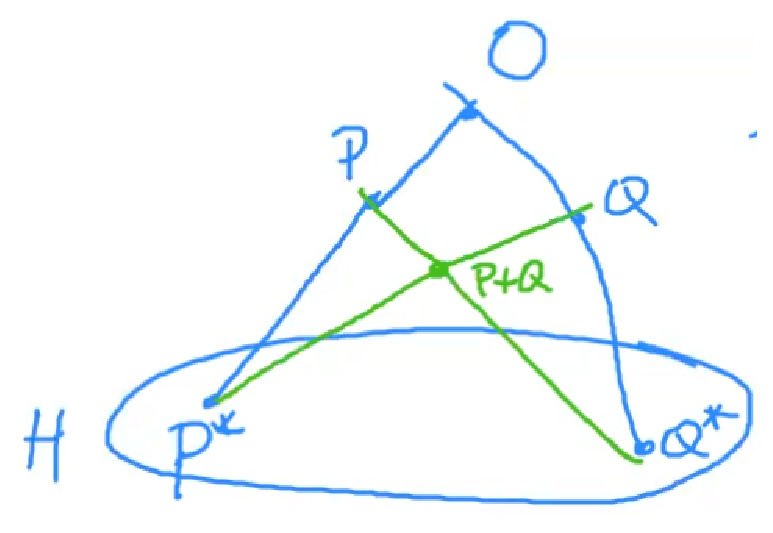
\includegraphics[scale=0.3]{g_24.eps}
\end{observation}

\begin{theorem}[$T(H)$ se skládáním a $P^*$ se sčítáním]
    $(T(H),\circ)\cong(\mathcal{P}^*,+)$
\end{theorem}
\begin{proof}
    Baerova věta \cref{kpp:baer} zajišťuje, že $P\rightarrow \tau_P$ je bijekce, a izomorfismus plyne z definice.
\end{proof}

\begin{note}
	Nulovým prvkem v $(P^*, +)$ je bod $O, \tau_O = id$.
	Opačný prvkem k $X$ je $-X$.
	Protože $(\tau_X)^{-1}(O)$ je kolineace, je $-X \in OX$.
	Pak pro všechna $X, Y \in P^*$ platí:
	\begin{gather*}
		\tau_{X + Y} = \tau_X \tau_Y\\
    		\tau_{-X} \circ \tau_X = id \Rightarrow \tau_{-X} = \tau_X^{-1}\\
		\tau_{-(X + Y)} = (\tau_X \tau_Y)^{-1} = \tau_X^{-1} \tau_Y^{-1} = \tau_{-Y}\tau_{-X} = \tau_{-Y + (-X)}\\
		\text{Tedy}\\
		-(X + Y) = (-X) + (-Y)
	\end{gather*}
\end{note}

\begin{definition}[Operace s kolineacemi, nula]
    Označme $\D_O$ množinu všech centrálních kolineací s osou $H$ a středem $O$.
    Dále označme $\omega$ zobrazení z $P$ do $P$, definované předpisem:
    \[ \omega(X) = \twopartdef{X}{X \in H}{O}{X \in P^*} \]
    %které $X$ zobrazí samo na sebe, je-li v ose a na $O$, je-li $X$ mimo osu.

    Na množině $F=\D_O\cup\{\omega\}$ definujeme sčítání a násobení následovně:
    \[ (\alpha+\beta)(X) = \twopartdef{X}{X \in H}{\alpha(X)+\beta(X)}{X \in P^*} \]
\end{definition}

\begin{observation}
	Pro každé $\alpha \in F$ platí:
	\begin{gather*}
		\alpha + \omega = \omega + \alpha = \alpha \\
		\alpha \cdot \omega = \omega \cdot \alpha = \omega
	\end{gather*}
\end{observation}

\begin{lemma}[O zobrazení $\mu$]
    Definujme zobrazení $\mu$ předpisem
    \[ \mu(X) = \twopartdef{X}{X \in H}{-X}{jinak} \]
    Pak $\mu\in \D_O$.
\end{lemma}
\begin{proof}
    Z definice $\mu$ fixuje každý bod nadroviny i střed $O$.
    Stačí tedy ukázat, že $\mu$ je kolineace dle \cref{kpp:equiv} -- neboť $\mu$ zachovává kolinearitu.
    Pro body ležící na přímce procházející bodem $O$ to je zjevné.
    Pro $g$ neprocházející bodem $O$ mějme $C=g\cap H$.
    Pak $g=\{P+X: X\in OC\}$ a
    \[ \mu(g) = \{\mu(P+X): X\in OC\} = \{-P+(-X):X\in OC\}=\{-P+Y: Y\in OC\}=-PC \]
\end{proof}
\begin{lemma}[Kolineace jsou automorfismy grupy]
    Každá kolineace $\alpha\in \D_O$ je automorfismus grupy $(P^*,+)$, neboli
	\begin{enumerate}
		\item $\alpha(O)=O$
		\item $\alpha(X+Y)=\alpha(Y)+\alpha(Y)$
		\item $\forall X,Y \in P^*: \alpha(-X)=-\alpha(X)$.
	\end{enumerate}
\end{lemma}
\begin{proof}~
	\begin{enumerate}
		\item $\alpha(O)=O$ je zřejmé.
		%\item $\alpha(X+Y)=\alpha(Y)+\alpha(Y)$
		%\item $\forall X,Y \in P^*: \alpha(-X)=-\alpha(X)$.
	\end{enumerate}
    TODO Lemma 9
\end{proof}

\begin{consequence}
	Pro každé $\alpha \in \D_O$ platí:
	\begin{gather*}
		\alpha \cdot \mu = \mu \cdot \alpha \\
		\alpha \cdot \mu + \alpha = \omega
	\end{gather*}
\end{consequence}

\begin{lemma}[Součet kolineací je v $F$]
    Pro každé dvě ne nutně různé kolineace $\alpha,\beta\in \D_O$ je $\alpha+\beta\in F$.
\end{lemma}
\begin{proof}
    TODO Lemma 10
\end{proof}

\begin{theorem}[Veblenova]
    Struktura $(F,+,\cdot)$ je konečné těleso o $q$ prvcích.
\end{theorem}
\begin{proof}~
	% idea 12 predn od 01:18:00
	\begin{enumerate}
		\item Podle \cref{kpp:kolin_group} je $\D_O = \mathrm{Col}(C,H)$ grupa vůči operaci $\circ$.
		\item Sčítání na $F$ \cref{kpp:sum_operation} tvoří komutativní grupu s nulovým prvkem $\omega$, přičemž opačným prvkem k $\alpha \in F$ je $\mu \alpha$.
		\item Je snadné ukázat, že operace $+$ a $\circ$ jsou svázány distributivními zákony.
		\item Velikost $F$.
	Zvolme pevně bod $P \in P^*\setminus \{O\}$.
	Podle \cref{kpp:centr_kolin_prop} je centrální kolineace $\alpha \in \D_O$ jednoznačně určena hodnotou $\alpha(P) \in OP$.
	Na přímce $OP$ je $q + 1$ bodů, z toho 2 nelze použít ($O$ a průsečík přímky $OP$ s nadrovinou $H$), takže máme $q - 1$ možností (včetně identické kolineace).
	Podle Baerovy věty \cref{kpp:baer} pro každou z těchto možností
centrální kolineace skutečně existuje a je jediná.
	Je tedy $|\D_O| = q - 1 \Rightarrow |F| = q$.
	\end{enumerate}

\end{proof}
\begin{consequence}[Řád KPP je mocnina prvočísla]
    KPP řádu $q$ dimenze $>2$ existuje právě tehdy, když $q$ je mocnina prvočísla.
\end{consequence}
